\documentclass[12pt]{article}
\usepackage{amsmath,amsthm,amssymb,hyperref,fancyhdr,color,multicol,enumitem}
\usepackage[margin=.5in,bottom=1in]{geometry}
\usepackage{pgfplots}
\pgfplotsset{compat=1.11}

\newcommand{\R}{\mathbb{R}}
\newcommand{\Z}{\mathbb{Z}}

\pagestyle{fancy} 
\fancyhf{}\renewcommand{\headrulewidth}{0pt}

\newcommand{\graphA}{
	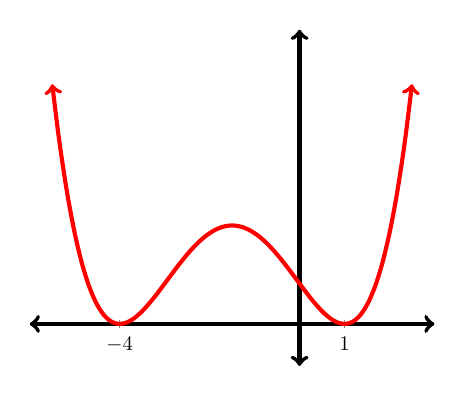
\begin{tikzpicture}[scale=.75]
		\begin{axis}[ 
		axis lines = middle,
		axis line style={<->},
		xmin=-6, xmax=3,
		ymin=-100, ymax=700,
		grid=none,
		xtick={-4,1},
		ytick=\empty,
		samples=50,
		smooth,
		no markers,
		domain=-5.5:2.5,
		line width=2pt
		]
		\addplot[<->,red] {6*(x+4)^2*(x-1)^2};
		\end{axis}
	\end{tikzpicture}
}
\newcommand{\graphB}{
	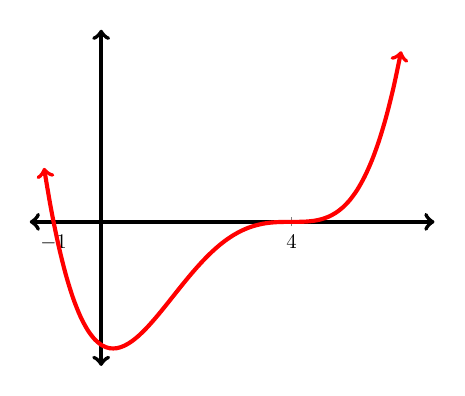
\begin{tikzpicture}[scale=.75]
		\begin{axis}[ 
		axis lines = middle,
		axis line style={<->},
		xmin=-1.5, xmax=7,
		ymin=-600, ymax=800,
		grid=none,
		%ticklabel style=left,
		xtick={4,-1},
		ytick=\empty,
		samples=50,
		smooth,
		no markers,
		domain=-1.2:6.3,
		line width=2pt
		]
		\addplot[<->,red] {8*(x-4)^3*(x+1)};
		\end{axis}
	\end{tikzpicture}
}
\newcommand{\graphC}{	
	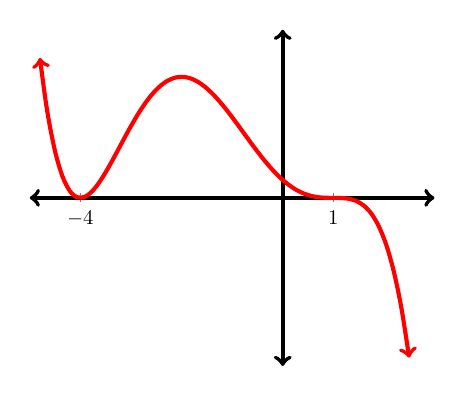
\begin{tikzpicture}[scale=.75]
		\begin{axis}[ 
			axis lines = middle,
			axis line style={<->},
			xmin=-5, xmax=3,
			ymin=-450, ymax=450,
			grid=none,
			xtick={-4,1},
			ytick=\empty,
			samples=50,
			smooth,
			no markers,
			domain=-4.8:2.5,
			line width=2pt
			]
			\addplot[<->,red] {-3*(x+4)^2*(x-1)^3};
		\end{axis}
	\end{tikzpicture}
}
\newcommand{\graphD}{
		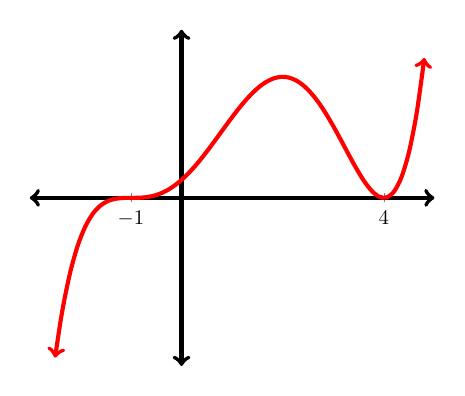
\begin{tikzpicture}[scale=.75]
		\begin{axis}[ 
			axis lines = middle,
			axis line style={<->},
			xmin=-3, xmax=5,
			ymin=-300, ymax=300,
			grid=none,
			xtick={4,-1},
			ytick=\empty,
			samples=50,
			smooth,
			no markers,
			domain=-2.5:4.8,
			line width=2pt
			]
			\addplot[<->,red] {2*(x-4)^2*(x+1)^3};
		\end{axis}
	\end{tikzpicture}
}
\newcommand{\graphE}{
	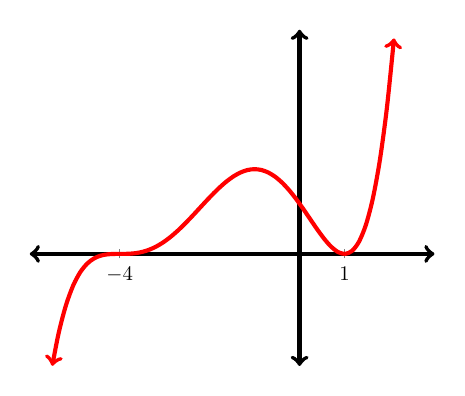
\begin{tikzpicture}[scale=.75]
		\begin{axis}[ 
			axis lines = middle,
			axis line style={<->},
			xmin=-6, xmax=3,
			ymin=-1000, ymax=2000,
			grid=none,
			xtick={-4,1},
			ytick=\empty,
			samples=50,
			smooth,
			no markers,
			domain=-5.5:2.1,
			line width=2pt
			]
			\addplot[<->,red] {7*(x+4)^3*(x-1)^2};
		\end{axis}
	\end{tikzpicture}
}
\newcommand{\graphF}{
		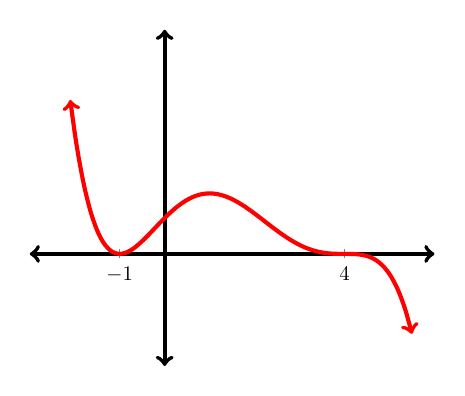
\begin{tikzpicture}[scale=.75]
		\begin{axis}[ 
			axis lines = middle,
			axis line style={<->},
			xmin=-3, xmax=6,
			ymin=-1000, ymax=2000,
			grid=none,
			xtick={4,-1},
			ytick=\empty,
			samples=50,
			smooth,
			no markers,
			domain=-2.1:5.5,
			line width=2pt
			]
			\addplot[<->,red] {-5*(x-4)^3*(x+1)^2};
		\end{axis}
	\end{tikzpicture}
}

\begin{document}
	\noindent Math 109: Algebra for Calculus\hfill Exam 3 Review\\
	\mbox{}\hfill Chapter 3: Polynomial Functions
	\setcounter{page}{1}
	\fancyfoot[C]{\thepage}
\begin{enumerate}
	\item Consider the parabola given by $f(x)=7x^2+10x-23$.
		\begin{enumerate}
			\item What is the vertex of the parabola?
			\vfill
			\item Does the parabola open up or down?\vfill
			\item What is the maximum or minimum value of the parabola?\vfill
			\item What is the axis of symmetry?\vfill
			\item Determine the $x$-intercept(s).\vfill
			\item Determine the $y$-intercept.\vfill
			\item Sketch a graph of the parabola.
				\vskip 2in
			\item What are the domain and range of the function?\vfill
		\end{enumerate}
	\newpage
	\item The monthly profit for a small company that makes long-sleeve T-shirts depends on the price per shirt. If the price is too high, sales will drop. If the price is too low, the revenue brought in may not cover the cost to produce the shirts. After months of data collection, the sales team determines that the  monthly profit is approximated by $f(p)=-50p^2+1700p-12000$, where $p$ is the price per shirt and $f(p)$ is the monthly profit based on the price.
		\begin{enumerate}
			\item Find the price that generates the maximum profit.
			\vskip 1in
			\item Find the maximum profit.
			\vskip 1in
			\item Find the price(s) that would enable the company to break even.
			\vskip 1in
		\end{enumerate}
	\item Describe the end behavior of the polynomial function 
		\begin{enumerate}
			\item $f(x)=9x^{4} + 129x^{3} + 201x^{2} + 645x + 780$
				\vfill
			\item $g(x)=-2x^{3} + x^{2} - x - 1$
				\vfill
			\item $h(x)=2x^{5} - 3x^{4} + 2x^{3} - x$
				\vfill
		\end{enumerate}
	\newpage
	\item Sketch a graph of the function
		\begin{enumerate}
			\item $g(x)=x^{3} + 6x^{2} + 5x$
			\vfill
			\item $h(x)=(2x-1)(x+1)^3$
			\vfill
		\end{enumerate}
	\newpage
	\item For each of (A)-(F) select the appropriate graph (I)-(VI) and give reasons why. 
		\begin{multicols}{2}
			\begin{enumerate}[label=(\Alph*)]
				\setlength{\itemsep}{.75in}
				\item[(A)] \underline{\hspace*{.25in}} $f(x)=2(x-4)^2(x+1)^3$
				\item[(C)] \underline{\hspace*{.25in}} $h(x)=-5(x-4)^3(x+1)^2$ 
				\item[(E)] \underline{\hspace*{.25in}} $q(x)=7(x+4)^3(x-1)^2$
				\item[(B)] \underline{\hspace*{.25in}} $g(x)=8(x-4)^3(x+1)$ 
				\item[(D)] \underline{\hspace*{.25in}} $p(x)=-3(x+4)^2(x-1)^3$
				\item[(F)] \underline{\hspace*{.25in}} $r(x)=6(x+4)^2(x-1)^2$
			\end{enumerate}
		\end{multicols}
		\vfill
		\begin{multicols}{2}
			\begin{enumerate}[label=(\Roman*)]
				\item[(I)] \begin{minipage}{2in}\graphA\end{minipage}
				\item[(III)] \begin{minipage}{2in}\graphD\end{minipage}
				\item[(V)] \begin{minipage}{2in}\graphC\end{minipage}
				\item[(II)] \begin{minipage}{2in}\graphB\end{minipage}
				\item[(IV)] \begin{minipage}{2in}\graphE\end{minipage}
				\item[(VI)] \begin{minipage}{2in}\graphF\end{minipage}
			\end{enumerate}
		\end{multicols}
	\newpage
	\item Use polynomial long division or synthetic division to write $\dfrac{f(x)}{g(x)}=q(x)+\dfrac{r(x)}{g(x)}$.  That is, find the quotient and the remainder.
		\begin{enumerate}
			\item $\dfrac{-3x^{5} - 10x^{3} + x^{2} - x}{x^{3} + 5}$
				\vfill
			\item $\dfrac{2x^{4} + 37x^{3} + 33x^{2} - 2x}{x+1}$
				\vfill
		\end{enumerate}
	\item
		Given the polynomial $9x^{3} + 6x^{2} - 5x - 2$ which of the following are linear factors of the polynomial?
			\begin{multicols}{2}
				\begin{enumerate}[label=(\Alph*)]\setlength{\itemsep}{2em}
					\item $x-1$
					\item $x+1$
					\item $x$
					\item $x-2$
					\item $x-\dfrac{2}{3}$
					\item $x-\dfrac{5}{13}$
				\end{enumerate}
			\end{multicols}
	\newpage
	\item
		What are the rational roots of the function $p(x)=2x^{4} + x^{3} + 9x^{2} + 5x - 5$?
		\vfill
%		\begin{enumerate}[label=(\Alph*)]\setlength{\itemsep}{2em}
%			\item $5$
%			\item $-5$
%			\item $\dfrac{5}{2}$
%			\item $-\dfrac{5}{2}$
%			\item $1$
%			\item $-1$
%			\item $\dfrac{1}{2}$
%			\item $-\dfrac{1}{2}$
%		\end{enumerate}
	\item Completely factor the polynomial $2 x^{3} - 15 x^{2} + 6 x + 7$.
		\vfill
		
		\newpage
	\item Find all roots of the polynomial $S(x)=4x^{3} - 5x^{2} - 3x + 1$.
		\vfill
	\item If $f(x)=-3x^{4} + x^{3} - 6x^{2} + 3x + 9$ and $i\sqrt{3}$ is a root of $f$, find all roots of $f$.
		\vfill
		\newpage
	\item What are the vertical asymptote(s) of $h(x)=\dfrac{x+2}{3x^{2} + 4x + 1}$?
		\vfill
	\item What are the horizontal asymptote(s) of $h(x)=\dfrac{x+2}{3x^{2} + 4x + 1}$?
		\vfill
	\item Sketch a graph of the function
		\begin{enumerate}
			\item $f(x)=\dfrac{5x-1}{8x+3}$
			\vfill\vfill\vfill\vfill
			\newpage
			\item $g(x)=\dfrac{2}{x^2+1}$
			\vfill
			\item $h(x)=\dfrac{3x^3}{x^2+7x-18}$
			\vfill
		\end{enumerate}
	\newpage
	\item Solve the inequality $2x^{2}\geq1-x$
	\vfill
	\item Solve the inequality $\dfrac{x+7}{x-3}<0$.
	\vfill
	\newpage
	
	\item For each Section in Chapter 3, write down the key terms and ideas.
	\begin{enumerate}
		\item Section 3.1: \vfill
		\item Section 3.2: \vfill
		\item Section 3.3: \vfill
		\newpage
		\item Section 3.4: \vfill
		\item Section 3.5: \vfill 
		\item Section 3.6: \vfill 
	\end{enumerate}
\end{enumerate}
\end{document}